% Created 2022-09-22 jue 13:56
% Intended LaTeX compiler: pdflatex
\documentclass[12pt]{article}
\usepackage[utf8]{inputenc}
\usepackage[T1]{fontenc}
\usepackage{graphicx}
\usepackage{grffile}
\usepackage{longtable}
\usepackage{wrapfig}
\usepackage{rotating}
\usepackage[normalem]{ulem}
\usepackage{amsmath}
\usepackage{textcomp}
\usepackage{amssymb}
\usepackage{capt-of}
\usepackage{hyperref}
\usepackage[spanish]{babel}
\usepackage{graphicx,geometry}
\geometry{ a4paper, left=1in, right=1in, top=1in, bottom=1in }
\renewcommand\familydefault{\sfdefault}
\usepackage{sectsty}
\sectionfont{\normalfont\Large }
\subsectionfont{\normalfont\normalsize}
\usepackage{tabularx}
\usepackage{listings}
\lstdefinestyle{mystyle}{
numbers=left,
showspaces=false,
frame=leftline,
showspaces=false,
showstringspaces=false,
showtabs=false,
numberstyle=\tiny,
}
\lstset{
style=mystyle,
literate={á}{{\'a}}1
{é}{{\'e}}1
{í}{{\'{\i}}}1
{ó}{{\'o}}1
{ú}{{\'u}}1
{Á}{{\'A}}1
{É}{{\'E}}1
{Í}{{\'I}}1
{Ó}{{\'O}}1
{Ú}{{\'U}}1
{ü}{{\"u}}1
{Ü}{{\"U}}1
{ñ}{{\~n}}1
{Ñ}{{\~N}}1
{¿}{{?``}}1
{¡}{{!``}}1
}
\makeatletter
\usepackage{fancyhdr}
\pagestyle{fancy}
\usepackage{mdframed}
\BeforeBeginEnvironment{minted}{\begin{mdframed}}
\AfterEndEnvironment{minted}{\end{mdframed}}
\author{Luis Eduardo Galindo Amaya (1274895)}
\date{22-09-2022}
\title{L1-Predicción}
\hypersetup{
 pdfauthor={Luis Eduardo Galindo Amaya (1274895)},
 pdftitle={L1-Predicción},
 pdfkeywords={},
 pdfsubject={},
 pdfcreator={Emacs 26.3 (Org mode 9.1.9)}, 
 pdflang={Spanish}}
\begin{document}


\newcommand{\docente}{Olivia Mendoza Duarte}
\newcommand{\asignatura}{Estadística Avanzada}
\newcommand{\semestre}{2022-2}

\newcommand{\miportada}[1]{
	\begin{titlepage}
		\vspace*{0.75in}
		\begin{flushleft}
			\sffamily
			\large #1       \\
			\Huge
            \@title         \\
			\hrulefill
			\vspace{0.25in} \\
			\Large \@author \\
			\vspace*{\fill}
            
\includegraphics[width=\textwidth]{../includes/filler.png} \\
			\vspace*{\fill}
			\large
			\begin{tabular}{|l|l|}
              \hline
			  Asignatura & \asignatura \\
			  Docente    & \docente    \\
			  Fecha      & \@date      \\
              \hline
			\end{tabular}
		\end{flushleft}
	\end{titlepage}
}

\miportada{ Práctica 5 }

\fancyhf{}
\lhead{ \asignatura }
\rhead{ \semestre }
\rfoot{Página \thepage}

\setlength\parindent{0pt}   % eliminar el intentado
\setlength{\parskip}{1.2em}

\maketitle
\end{center}

\section*{Instrucciones}
\label{sec:org96a08bb}
En ésta práctica usarás como base el ejemplo de regresión lineal simple en R visto en clase, para resolver un problema de predicción, mismo que propondrás del sitio del repositorio de la UCI (elegir un dataset distinto de las anteriores prácticas).

Entregarás el archivo con el código en R, capturas de pantalla de los resultados y una explicación del problema y la solución.

\section*{Dataset}
\label{sec:orgde34008}
\subsection*{Breast Cancer Wisconsin (Diagnostic)}
\label{sec:org239a900}
\begin{itemize}
\item 1. ID number
\item 2. Diagnosis (M = malignant, B = benign)
\end{itemize}

\subsection*{Ten real-valued features are computed for each cell nucleus:}
\label{sec:org1daa7fe}
\begin{itemize}
\item a. radius (mean of distances from center to points on the perimeter)
\item b. texture (standard deviation of gray-scale values)
\item c. perimeter
\item d. area
\item e. smoothness (local variation in radius lengths)
\item f. compactness (perimeter\(^{\text{2}}\) / area - 1.0)
\item g. concavity (severity of concave portions of the contour)
\item h. concave points (number of concave portions of the contour)
\item i. symmetry
\item j. fractal dimension ("coastline approximation" - 1)
\end{itemize}

\href{https://archive-beta.ics.uci.edu/ml/datasets/breast+cancer+wisconsin+diagnostic}{Origen}

\section*{Descripcion del problema}
\label{sec:org0f13e39}
Se espera encontrar una relacion entre el tamaño del tumor y su radio, los datos del dataset son compuestas de multiples mediciones. por lo que son un aproximado del tamaño del tumor.

\section*{Código R}
\label{sec:org07511ed}
\begin{verbatim}
archivo = read.csv("./dataset/wdbc.data", nrows = 30)
x = archivo[3] #radio
y = archivo[5] #perimetro

datos = data.frame(x,y)
datos
regresion = lm(datos)

b= regresion$coefficients[1]
m = regresion$coefficients[2]
b
m

yr = m * x + b
yr
datos_r = data.frame(x,yr)
datos_r

jpeg(file="img/rp.jpeg")
par(mfrow = c(2,1))
plot(datos)
plot(datos_r, type="l")
dev.off()

\end{verbatim}

\begin{figure}[htbp]
\centering
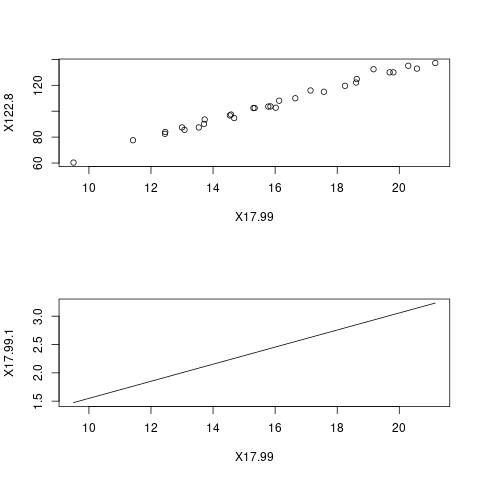
\includegraphics[width=10cm]{img/rp.jpeg}
\caption{'y' Radio del tumor, 'x' perimetro.}
\end{figure}

\section*{Regrecion resultante}
\label{sec:orgfc89c82}
\[ 0.1441553 x - 0.807 \]

\begin{center}
\begin{tabular}{rrr}
 & x2 & y\(_{\text{pred}}\)\\
\hline
1 & 1 & 0.9525883\\
2 & 2 & 1.0972761\\
3 & 3 & 1.2419639\\
4 & 4 & 1.3866517\\
5 & 5 & 1.5313394\\
6 & 6 & 1.6760272\\
23 & 23 & 4.1357197\\
24 & 24 & 4.2804075\\
25 & 25 & 4.4250953\\
\end{tabular}
\end{center}

\begin{verbatim}
archivo = read.csv("./dataset/wdbc.data")

x = archivo[1:300,3] #radio
y = archivo[1:300,5] #perimetro

datos = data.frame(x,y)
regresion = lm(datos)

b = regresion$coefficients[1]
m = regresion$coefficients[2]
yr = m * x + b

datos_r = data.frame(x,yr)
datos_r

## x2 = archivo[30:100,3] #radio
x2 = 1:300
y_pred = m * x2 + b


jpeg(file="img/rp2.jpeg")
par(mfrow = c(3,1))
plot(datos)
plot(datos_r, type="l")
plot(y_pred, type="l")
dev.off()
\end{verbatim}

\begin{figure}[htbp]
\centering
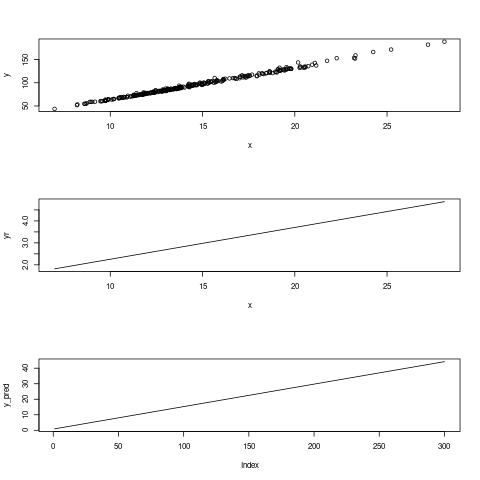
\includegraphics[width=10cm]{img/rp2.jpeg}
\caption{'y' Radio del tumor, 'x' perimetro}
\end{figure}
\end{document}
